\documentclass[nobib]{tufte-handout}

%\\geometry{showframe}% for debugging purposes -- displays the margins

\newcommand{\bra}[1]{\left(#1\right)}
\usepackage{amssymb}
\usepackage{hyperref}
\usepackage[activate={true,nocompatibility},final,tracking=true,kerning=true,spacing=true,factor=1100,stretch=10,shrink=10]{microtype}
\usepackage{color}

% Fixes captions and images being cut off
\usepackage{marginfix}
\usepackage{array}
\usepackage{tikz}
\usepackage{amsmath,amsthm}
\usetikzlibrary{shapes}
\usetikzlibrary{positioning}
\usepackage{listings}
\usepackage{caption}
\DeclareCaptionFont{white}{\color{white}}
\DeclareCaptionFormat{listing}{\colorbox{gray}{\parbox{\textwidth}{#1#2#3}}}
\captionsetup[lstlisting]{format=listing,labelfont=white,textfont=white}

% Set up the images/graphics package
\usepackage{graphicx}
\setkeys{Gin}{width=\linewidth,totalheight=\textheight,keepaspectratio}
\graphicspath{{.}}

\title{Notes for ECE 29595PD - Principles of Digital System Design}
\author[Shubham Saluja Kumar Agarwal]{Shubham Saluja Kumar Agarwal}
\date{\today}  % if the \date{} command is left out, the current date will be used

% The following package makes prettier tables.  We're all about the bling!
\usepackage{booktabs}

% The units package provides nice, non-stacked fractions and better spacing
% for units.
\usepackage{units}

% The fancyvrb package lets us customize the formatting of verbatim
% environments.  We use a slightly smaller font.
\usepackage{fancyvrb}
\fvset{fontsize=\normalsize}

% Small sections of multiple columns
\usepackage{multicol}

% For finite state machines 
\usetikzlibrary{automata} % Import library for drawing automata
\usetikzlibrary{positioning} % ...positioning nodes
\usetikzlibrary{arrows} % ...customizing arrows
\tikzset{node distance=2.5cm, % Minimum distance between two nodes. Change if necessary.
    every state/.style={ % Sets the properties for each state
    semithick,
    fill=gray!10},
    initial text={}, % No label on start arrow
    double distance=2pt, % Adjust appearance of accept states
    every edge/.style={ % Sets the properties for each transition
    draw,
    ->,>=stealth', % Makes edges directed with bold arrowheads
    auto,
    semithick}}
\let\epsilon\varepsilon

% These commands are used to pretty-print LaTeX commands
\newcommand{\doccmd}[1]{\texttt{\textbackslash#1}}% command name -- adds backslash automatically
\newcommand{\docopt}[1]{\ensuremath{\langle}\textrm{\textit{#1}}\ensuremath{\rangle}}% optional command argument
\newcommand{\docarg}[1]{\textrm{\textit{#1}}}% (required) command argument
\newenvironment{docspec}{\begin{quote}\noindent}{\end{quote}}% command specification environment
\newcommand{\docenv}[1]{\textsf{#1}}% environment name
\newcommand{\docpkg}[1]{\texttt{#1}}% package name
\newcommand{\doccls}[1]{\texttt{#1}}% document class name
\newcommand{\docclsopt}[1]{\texttt{#1}}% document class option name

% Define a custom command for definitions and biconditional
\newcommand{\defn}[2]{\noindent\textbf{#1}:\ #2}
\let\biconditional\leftrightarrow

\begin{document}

\maketitle

\begin{abstract}
    These are lecture notes for spring 2024 ECE 29595PD at Purdue. Modify, use, and distribute as you please.
\end{abstract}

\tableofcontents

\section{Course Introduction}

This course serves as an introduction to digital system design, with an
emphasis on principles of digital hardware and embedded system design. It is an
alternate class to ECE 27000. \\ Learning Outcomes:
\begin{enumerate}
    \item Ability to analyze and design combinational logic circuits.
    \item Ability to analyze and design sequential logic circuits.
    \item Ability to analyze and design computer logic circuits.
    \item Ability to realize, test, and debug practical digital circuits.
\end{enumerate}

\pagebreak

\section{Introduction}

Digital design entails creating hardware that can conduct an operation or set
of operations within a computer system. For example, adding two numbers. \\
\begin{center}
    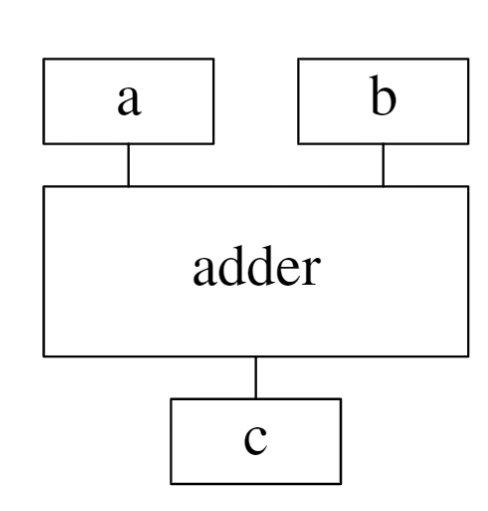
\includegraphics[width= 100px]{images/Screenshot 2024-01-08 151414.png}
\end{center}
This hardware can add two numbers, that is, conduct the operation $c=a+b$. It could also perform $f=d+e$ or $i=g-h=g+(-h)$ as it is not restricted to the sole values of $a$ and $b$ as inputs. This process fits into the logic design and switching algebra portions of chip manufacturing.\\
The creation of systems like these is based on the fact that voltage and current are time-varying and can assume any value in a continuous range of real numbers, but are mapped to only two values.

\subsection{Digital Logic Signals}
A digital signal is modeled as assuming, at anytime, only one of two discrete
values, which represent:\\
\begin{table}
    \centering
    \begin{tabular}{c|c}
        0     & 1    \\
        LOW   & HIGH \\
        FALSE & TRUE \\
    \end{tabular}
\end{table}
This is called positive logic.
This maps the infinite values of voltage and current to the two values.
An example of this is CMOS 2-Volt logic:\\
\begin{table}
    \centering
    \begin{tabular}{c|c}
        0      & 1        \\
        \hline
        0-0.5V & 1.5-2.0V \\
    \end{tabular}
\end{table}
These completely separated ranges of values allow for 0 and 1 to be completely separate, with noise and other possible errors being ignored. In this way, all physical values can be partitioned into the two values, though, for intents and purposes of digital system design, voltage is the most relevant.\\
Additionally, circuits known as buffer circuits can be used to restore logic values. That is, if a voltage is not sufficiently close to the values of 0 or 2 (in the case of the CMOS), they can push these values far closer to the desired values, reducing teh possibility of error.\\
Digital circuits have replaced analog circuits becuse they are far easier to design. They can be made using Hardware Description Languages (HDLs), softwares that are similar to programming languages.\\
A logic value is called a binary digit, or bit. A set of $n$ bits, represent $2^n$ values. For example:
\begin{table}
    \centering
    \begin{tabular}{c}
        $b_0$ \\
        \hline
        0     \\
        1     \\
    \end{tabular}
    \\
    \begin{tabular}{c c}
        $b_0$ & $b_1$ \\
        \hline
        0     & 0     \\
        1     & 0     \\
        0     & 1     \\
        1     & 1
    \end{tabular}
\end{table}
\subsection{Logic Circuits}
At the highest level, a logic circuit is a \textit{black box} with $n$ input
and $m$ outputs. Only zeros and ones are required to represent inputs and
outputs. \\ Combinational circuits are circuits that have outputs that solely
depend on the inputs. It can be represented by a truth table.\\ An adder can be
represented by a truth table in this manner.
\begin{center}
    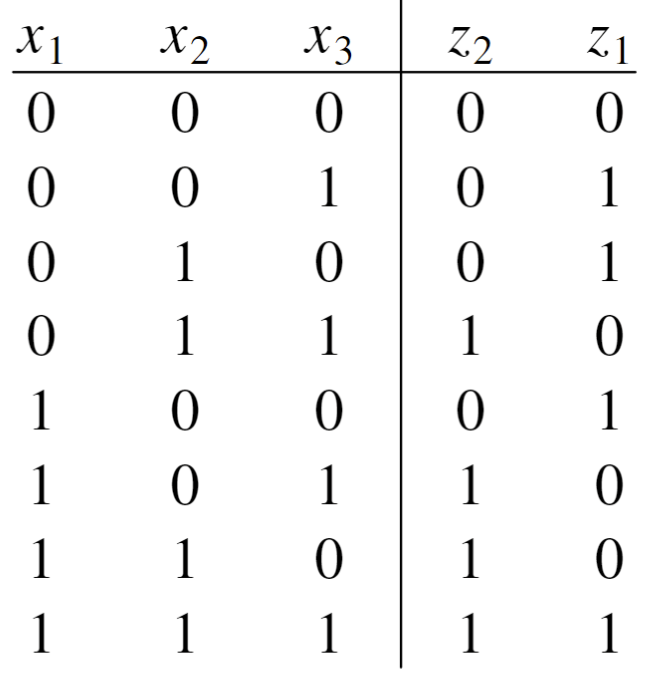
\includegraphics[width= 100px]{images/Screenshot 2024-01-10 144557.png}
\end{center}
On the other hand, a sequential circuit has memory. That is, the output is dependent on both the inputs and the current state of the circuit itself. This is representable through a state table.\\
\begin{center}
    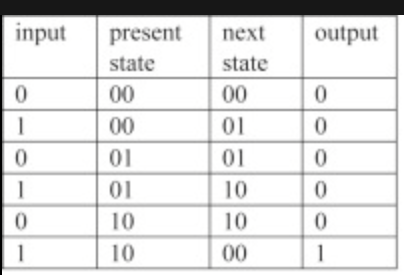
\includegraphics[width= 150px]{images/state table.png}
\end{center}
\subsection{Gates}
Basic digital devices are called gates. These implement basic logic functions.
These are AND, OR, NOT. However, AND, NOT and OR, NOT are sufficient to make
any combination, as the third gate can be formed as a combination of the other
two.\\ Each of the gates is represented symbolically like the following, and
have their truth tables shown below:\\
\begin{table}
    \centering
    \begin{tabular}{c|c|c}
        AND                                                & OR                                                & NOT                                                \\
        \hline
        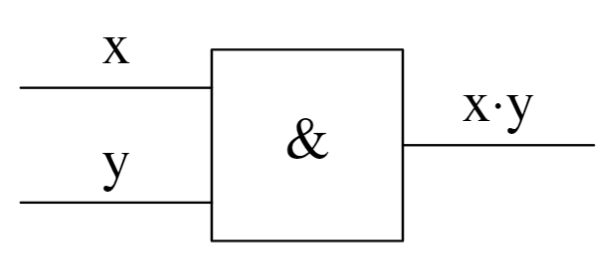
\includegraphics[width= 80px]{images/AND_GATE.png} & 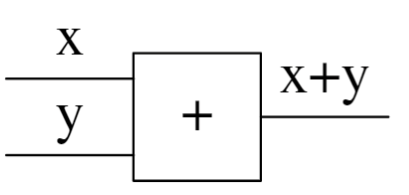
\includegraphics[width= 80px]{images/OR_GATE.png} & 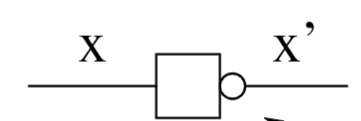
\includegraphics[width= 80px]{images/INVERTER.png} \\
        \hline
        \begin{tabular}{c c|c}
            x & y & {$x\land y$} \\
            \hline
            0 & 0 & 0            \\
            0 & 1 & 0            \\
            1 & 0 & 0            \\
            1 & 1 & 1
        \end{tabular}                            &
        \begin{tabular}{c c|c}
            x & y & {$x\lor y$} \\
            \hline
            0 & 0 & 0           \\
            0 & 1 & 1           \\
            1 & 0 & 1           \\
            1 & 1 & 1
        \end{tabular}                             &
        \begin{tabular}{c|c}
            x & {$\lnot x$} \\
            \hline
            0 & 1           \\
            1 & 0           \\
        \end{tabular}
    \end{tabular}
\end{table}
This can be done for more inputs, by combining multiple gates.\\ There are two more often used gates that can be created through a combination of these two.\\
\begin{table}
    \centering
    \begin{tabular}{c|c}
        NAND                                                & NOR                                                \\
        \hline
        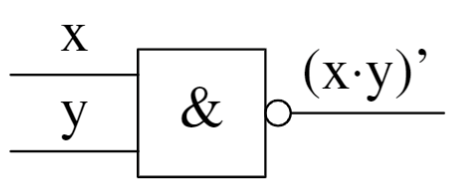
\includegraphics[width= 80px]{images/NAND_GATE.png} & 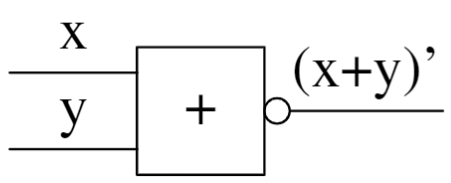
\includegraphics[width= 80px]{images/NOR_GATE.png} \\
        \hline
        \begin{tabular}{c c|c}
            x & y & {$\lnot(x\land y)$} \\
            \hline
            0 & 0 & 1                   \\
            0 & 1 & 0                   \\
            1 & 0 & 0                   \\
            1 & 1 & 0
        \end{tabular}                &
        \begin{tabular}{c c|c}
            x & y & {$\lnot(x\lor y)$} \\
            \hline
            0 & 0 & 1                  \\
            0 & 1 & 1                  \\
            1 & 0 & 1                  \\
            1 & 1 & 0
        \end{tabular}
    \end{tabular}
\end{table}
It is a good exercise to see how two of the basic gates (AND, NOT or OR, NOT) can be used to create the rest.\\
It is possible to connect gates to form complex circuits and thus, complex functions. By convention, signal flows from left to right. Thus, output comes out the right and input goes in at left.

\pagebreak
\end{document}